\chapter{Event Selection}
\label{chap:Evt}

Events are required to contain exactly two \emph{tight} leptons and one \emph{tight} tau, described in \autoref{chap:Obj}. A combination of single- and di-lepton \ac{HLT} triggers are used to select data as well as simulated events. The sum of the electric charges of all three leptons are required to be 1 or -1, which guarantees at lease one \ac{OSDF} pair in every selected event. Depending on the flavors and the charge assignments of the two leptons, events are further categorized into 6 different channels, which is described in \autoref{sec:Cat}. \acp{SR} require additional selection criteria to achieve an optimal signal to background ratio, which is discussed in \autoref{sec:SRInclusive}. Control regions of the \ac{DY} background near the Z resonance are also defined to study the accuracy of the \ac{MC} modeling, which is described in \autoref{sec:DY_CR}. 
%%%%%%%%%%%%%%%%%%%%%%%%%%%%%%%%%%%%%%%%%%%%%%%%%%
%%%%%%%%%%%%%%%%%%%%%%%%%%%%%%%%%%%%%%%%%%%%%%%%%%
\section{Event Categorization}
\label{sec:Cat}

The two \emph{tight} leptons can come with any flavor- or charge-compositions, which contain 6 possibilities: i) \ac{OS}-ee, ii) \ac{OS}-e$\upmu$, iii) \ac{OS}-$\upmu\upmu$, iv) \ac{SS}-ee, v) \ac{SS}-e$\upmu$, and vi) \ac{SS}-$\upmu\upmu$. These subsets of the selected events are referred to as ``channels'' in this analysis. The \ac{OS}-e$\upmu$ and \ac{SS}-e$\upmu$ channels are further subdivided into ``subchannels'' as more than one charged-lepton flavor mixing mode is possible in these channels. For example, due to the requirement on the sum of electric charges, the sign of the selected tau must be different from the signs of the electron and muon in the \ac{SS}-e$\upmu$ channel. This means both the e$\uptau$ and $\upmu\uptau$ flavor mixing modes are possible under such scenario. This two-fold ambiguity is resolved by using the existing strategy described in \autoref{sec:Kin}: two \ac{SM} quark candidates are reconstructed by combining the \ac{MET}, the jet with the highest \DeepJ score, and two leptons in question. The lepton that gives a top quark mass that is the closer to 172.5 GeV is designated as the standalone lepton while the other lepton is designated as the LFV lepton that contributes to the flavor mixing. There is only one subchannel for each of the other four channels as there is no ambiguity on which flavor mixing mode to designate for these channels. A total of 9 subchannels are defined, which is illustrated in Figure~\ref{fig:EvtCat}. 

As is shown in \ref{fig:SigGen}, the invariant mass of the LFV-dilepton pair of any mixing mode, denoted by m($\ell\ell^{\prime}$), has a sharp end point at around 150 GeV for top quark decay signals. Such a pattern does not exit in the top quark production signals. Therefore, each subchannel is further subdivided into two mass bins to create regions enriched in different signal modes using a threshold of 150 GeV on m($\ell\ell^{\prime}$), which is consistent with the strategy used in the previous analysis.

\begin{figure}[tbh!]
 \begin{center}
 \begin{tabular}{c}
 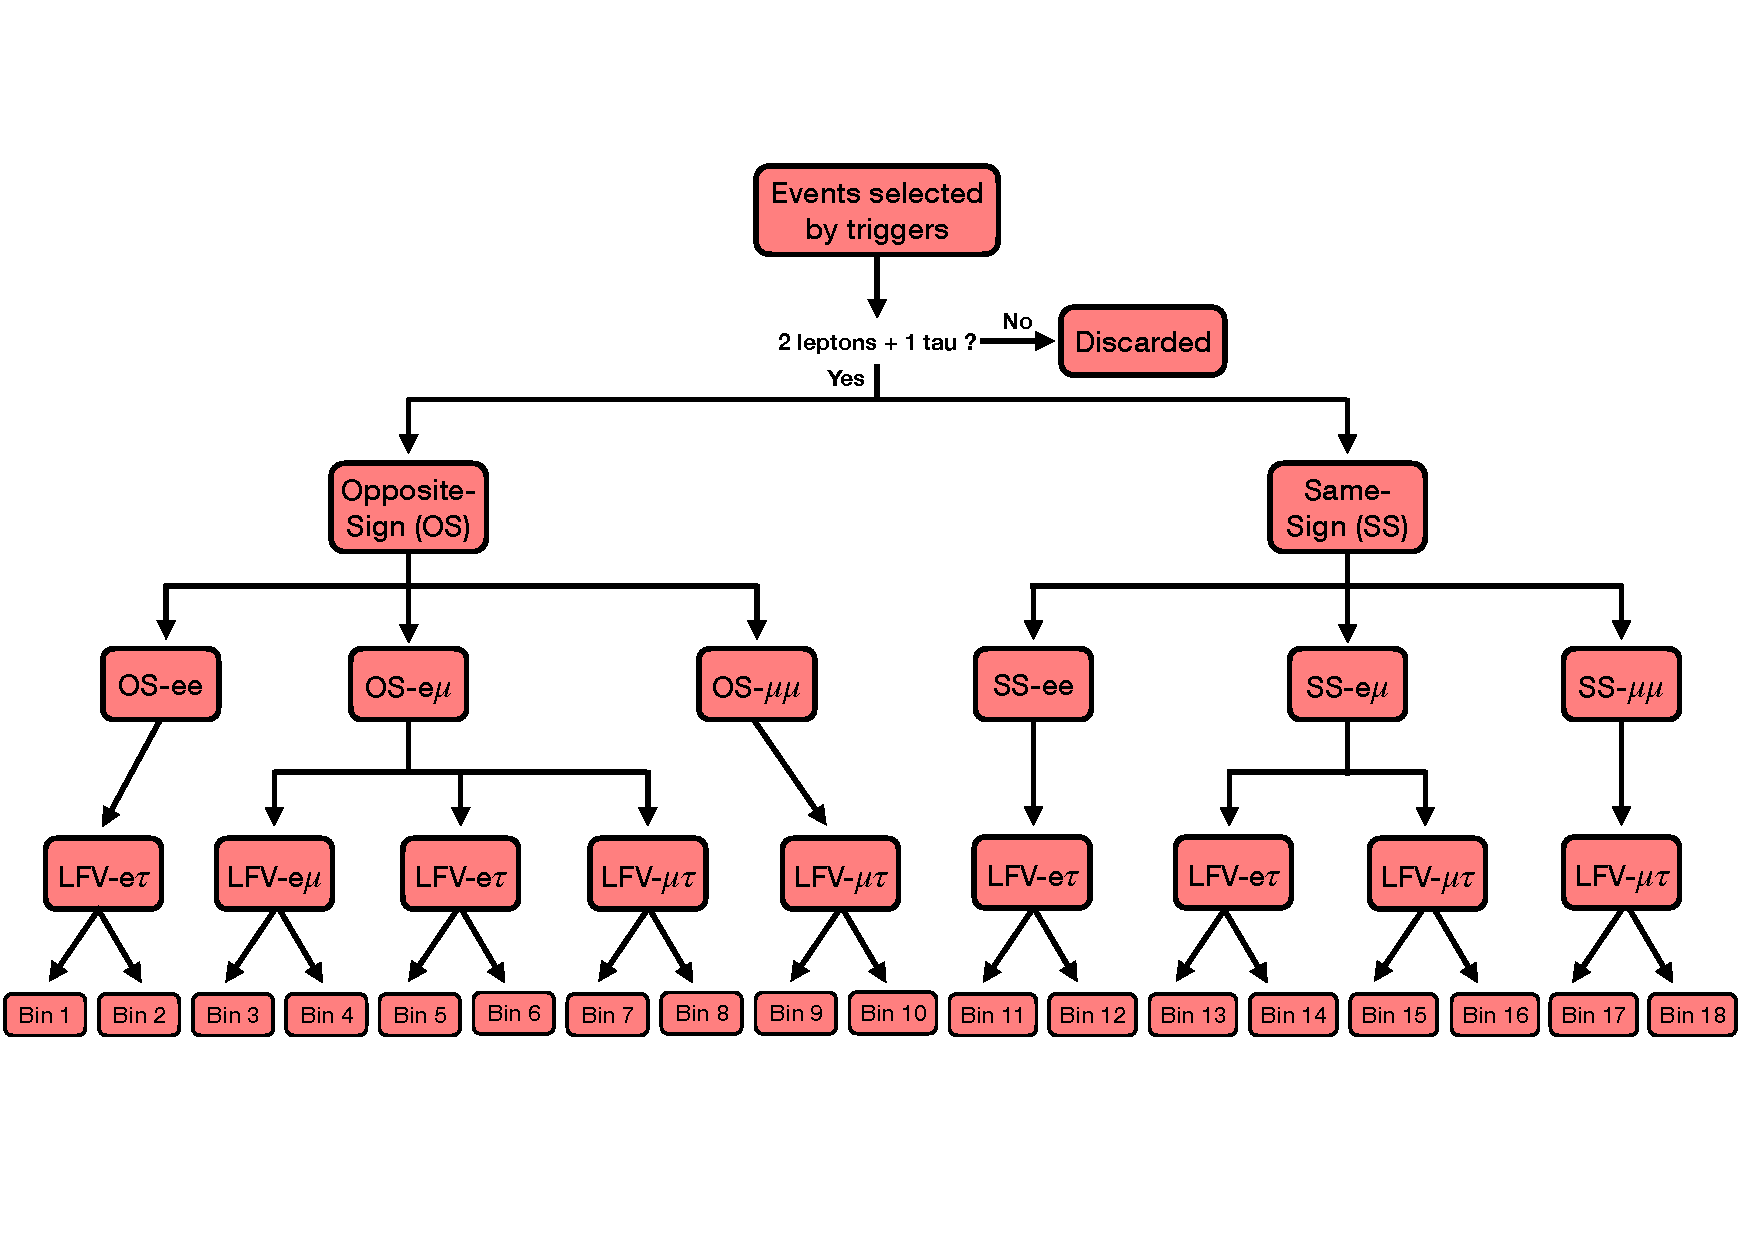
\includegraphics[width=\textwidth]{figures/Part4/Evt/SRFlowChart}
 \end{tabular}
 \caption{Illustration of event categorization scheme used by this analysis. The second to the last row shows 9 exclusive subchannels, where a specific charged-lepton flavor mixing mode is designated. The odd (even) bins shown in the last row correspond to mass bins with the requirement of m($\ell\ell^{\prime}$) $<(>)$ 150 GeV.}
 \label{fig:EvtCat}
 \end{center}
 \end{figure}
 
 The performance of this categorization scheme is evaluated by using simulated signal events that contain all three flavor mixing modes. Whether or not events are assigned to the wrong category is determined by using the generator-level information. The rate of occurrences of an incorrect assignment is largely under control, as is shown in Figure~\ref{fig:SRbin}. Further improvement is possible with the assistance from more sophisticated algorithms, such as \acp{NN}. 
 
 \begin{figure}[tbh!]
 \begin{center}
 \begin{tabular}{c}
 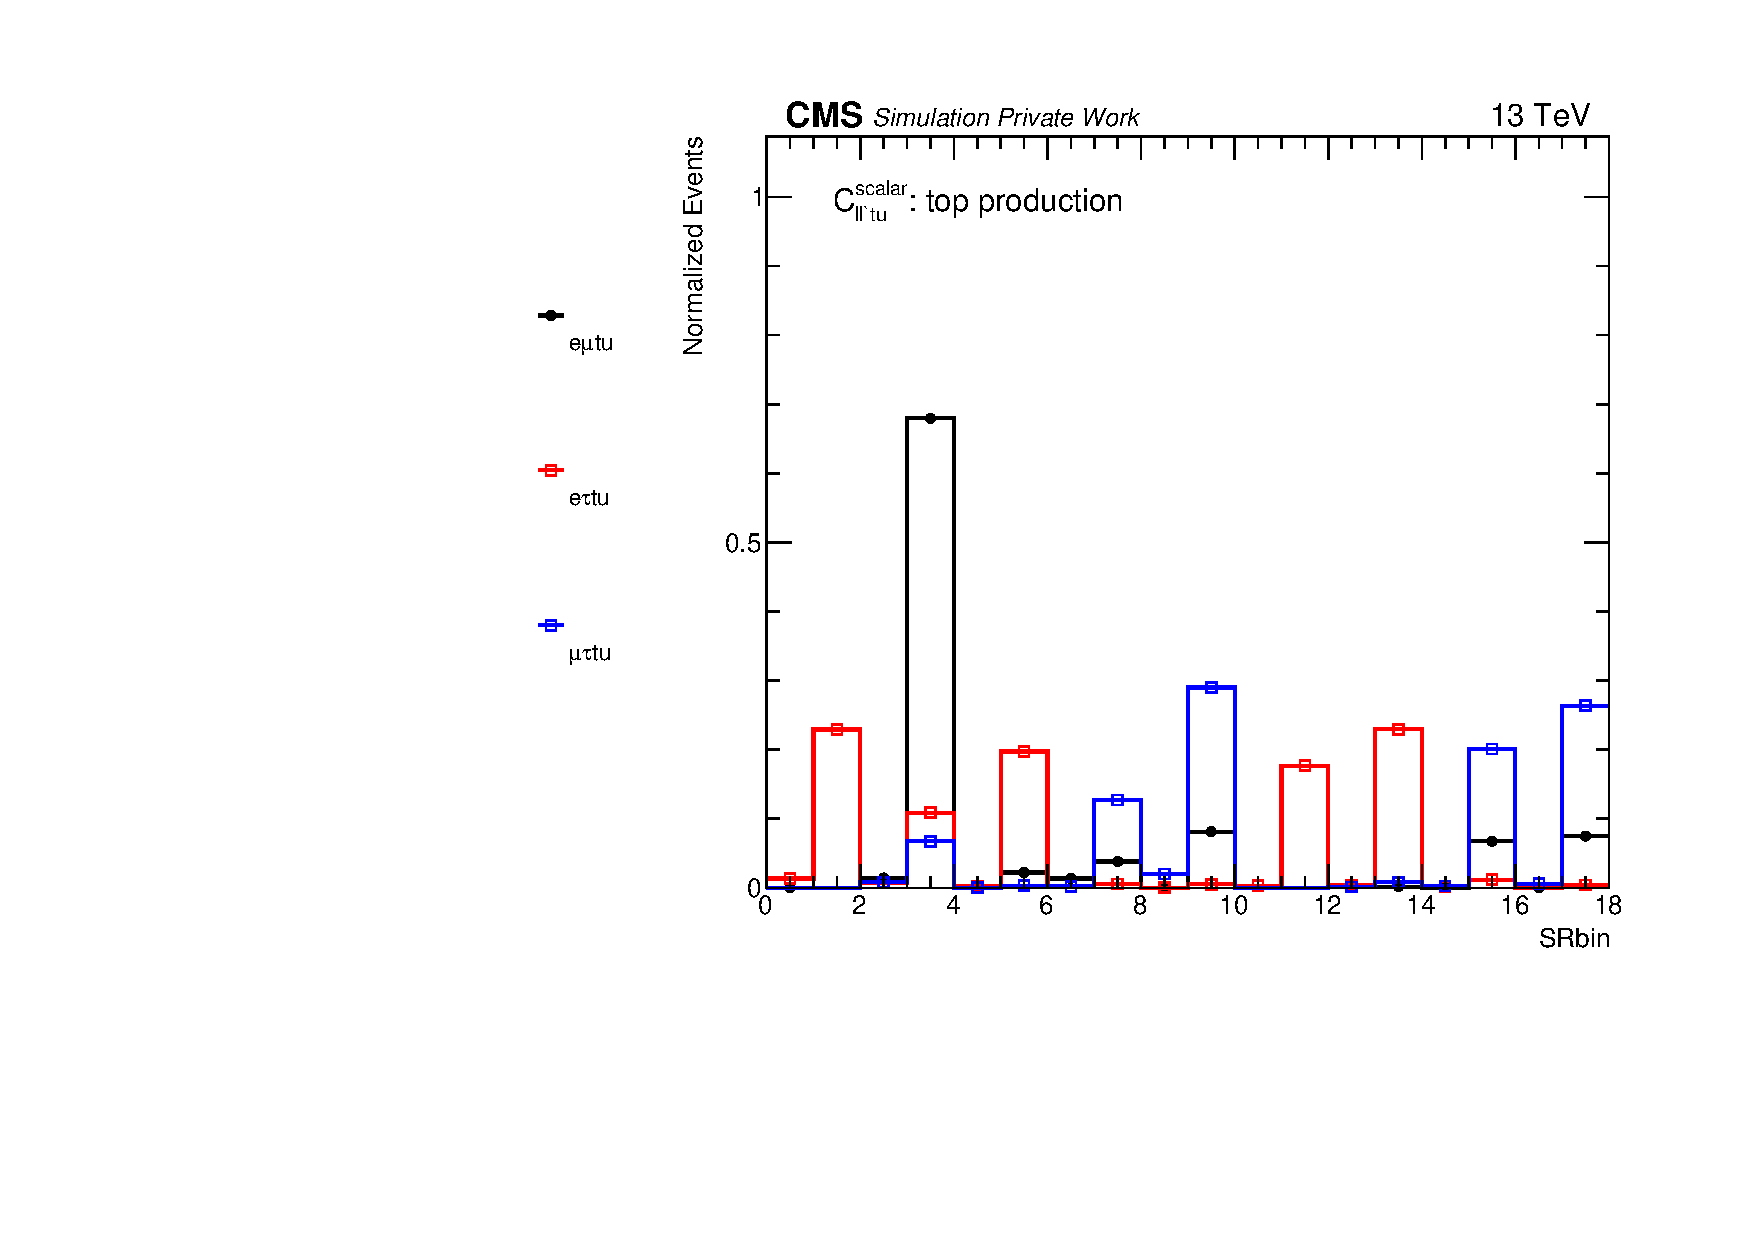
\includegraphics[width=0.8\textwidth]{figures/Part4/Evt/SRbin}
 \end{tabular}
 \caption{XX}
 \label{fig:SRbin}
 \end{center}
 \end{figure}
%%%%%%%%%%%%%%%%%%%%%%%%%%%%%%%%%%%%%%%%%%%%%%%%%%
%%%%%%%%%%%%%%%%%%%%%%%%%%%%%%%%%%%%%%%%%%%%%%%%%%

\section{Signal Region}
\label{sec:SRInclusive}

\begin{figure}[tbh!]
 \begin{center}
 \begin{tabular}{c}
 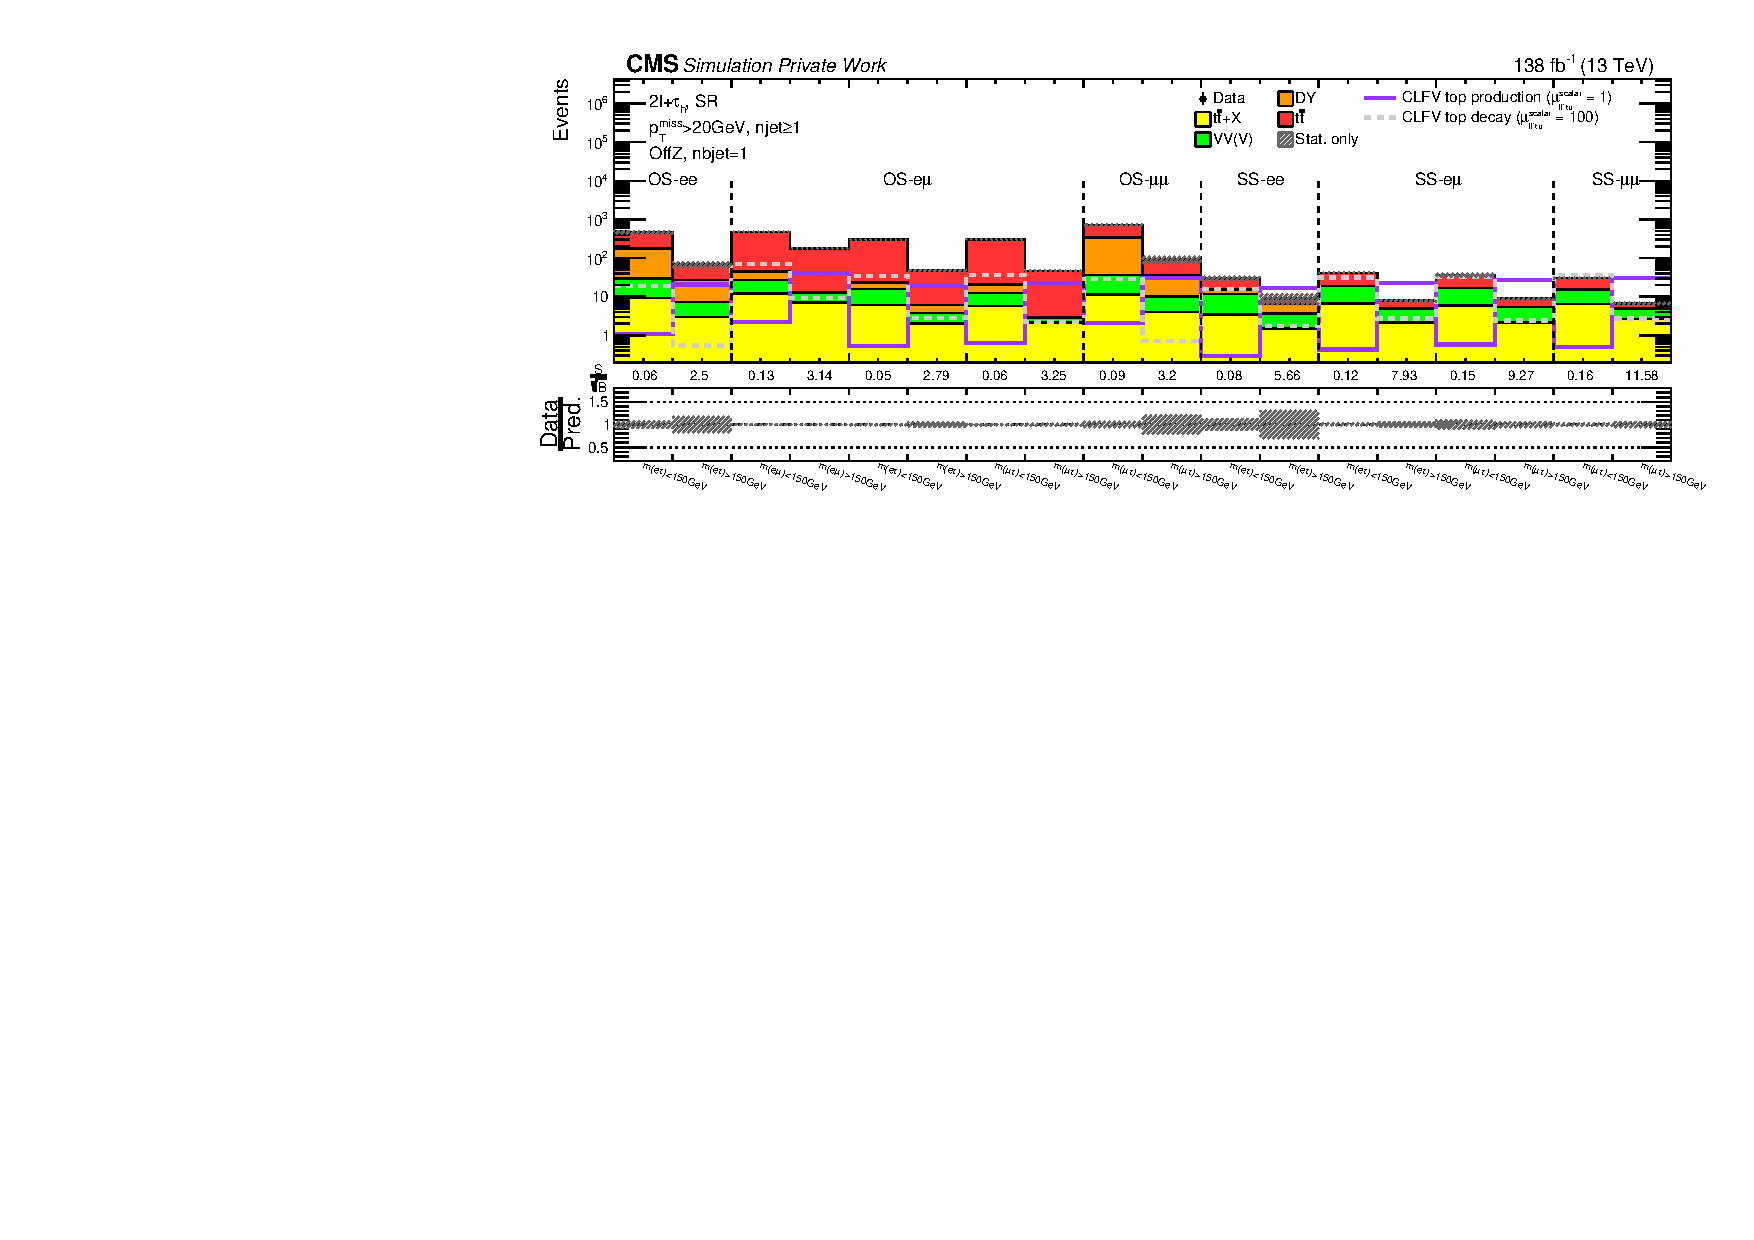
\includegraphics[width=\textwidth]{figures/Part4/Evt/Summary_llOffZMetg20B1}
 \end{tabular}
 \caption{XX}
 \label{fig:Summary}
 \end{center}
 \end{figure}
 
 \begin{figure}[tbh!]
 \begin{center}
 \begin{tabular}{ccc}
 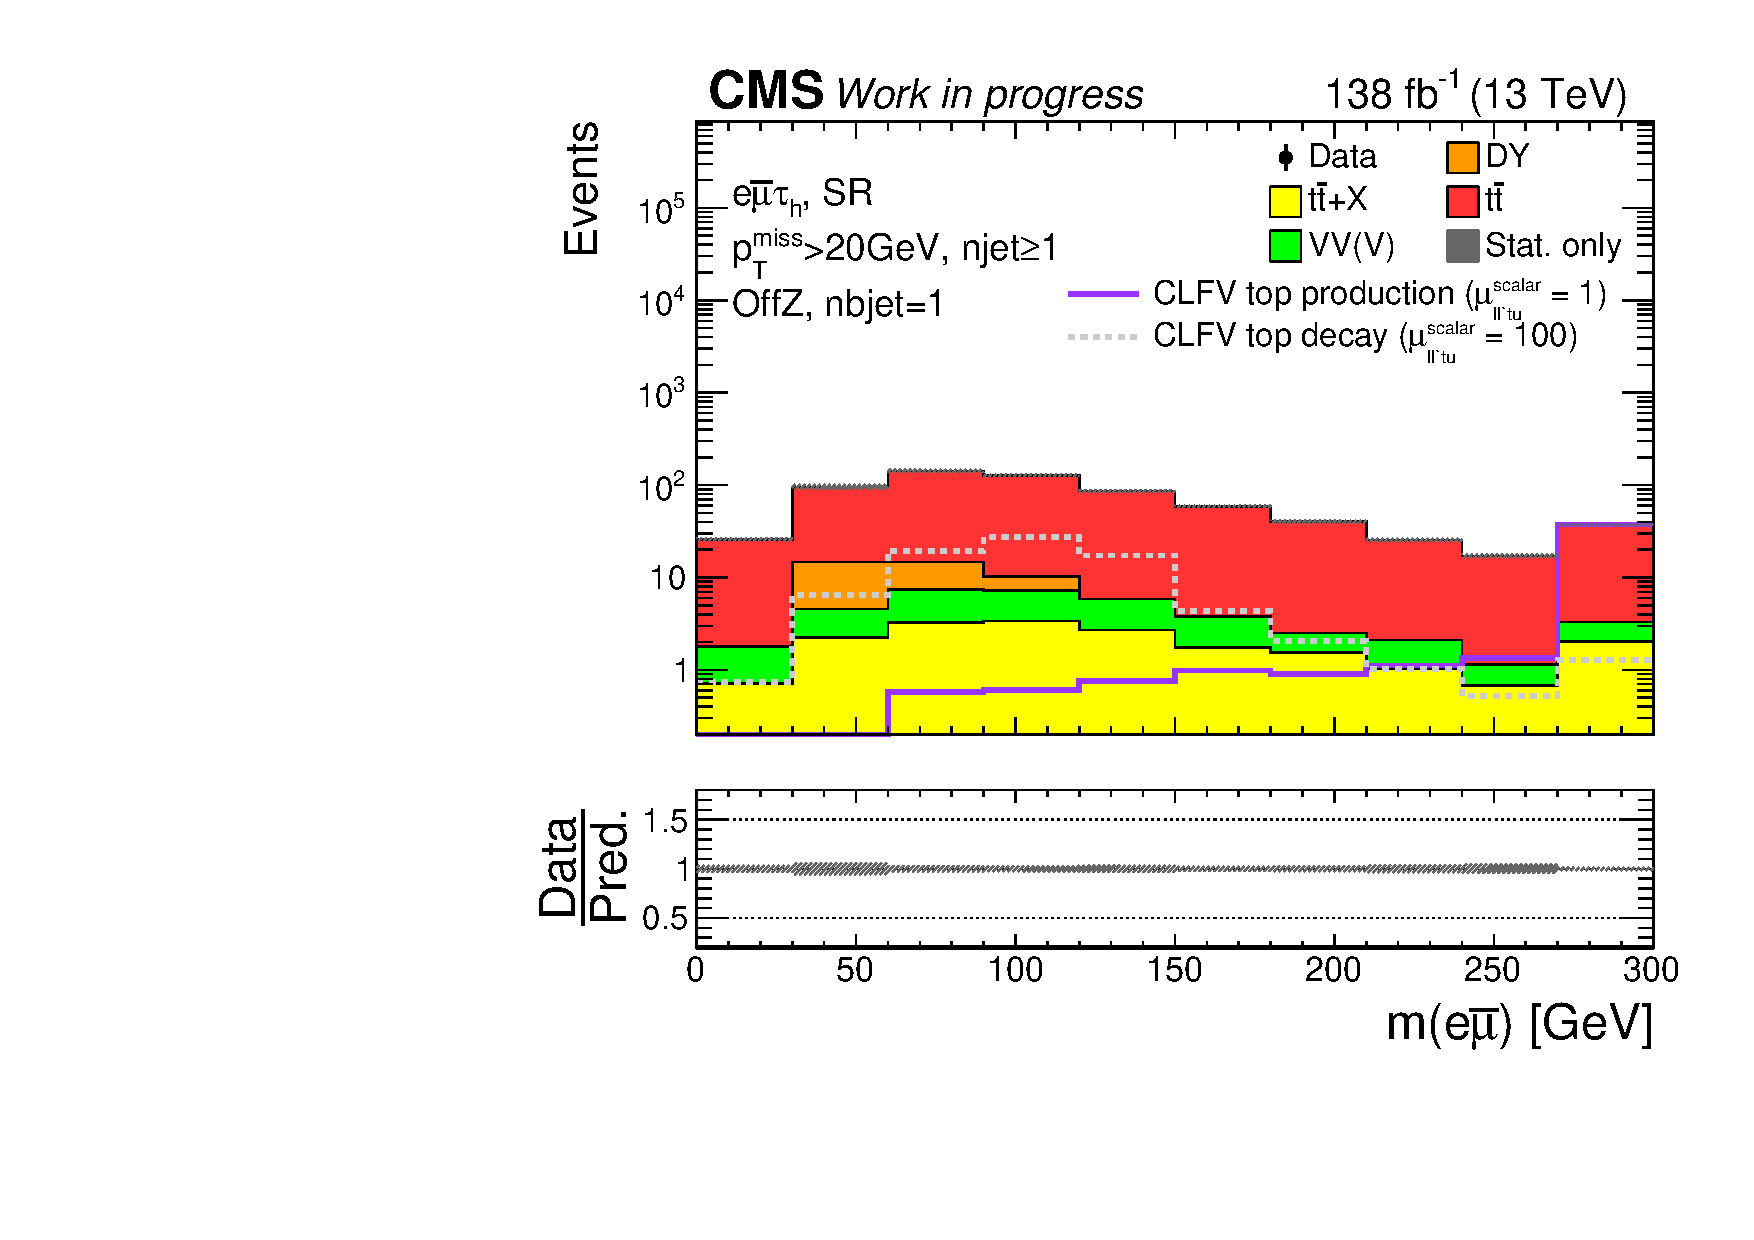
\includegraphics[width=0.33\textwidth]{figures/Part4/Evt/LFVemuM}&
 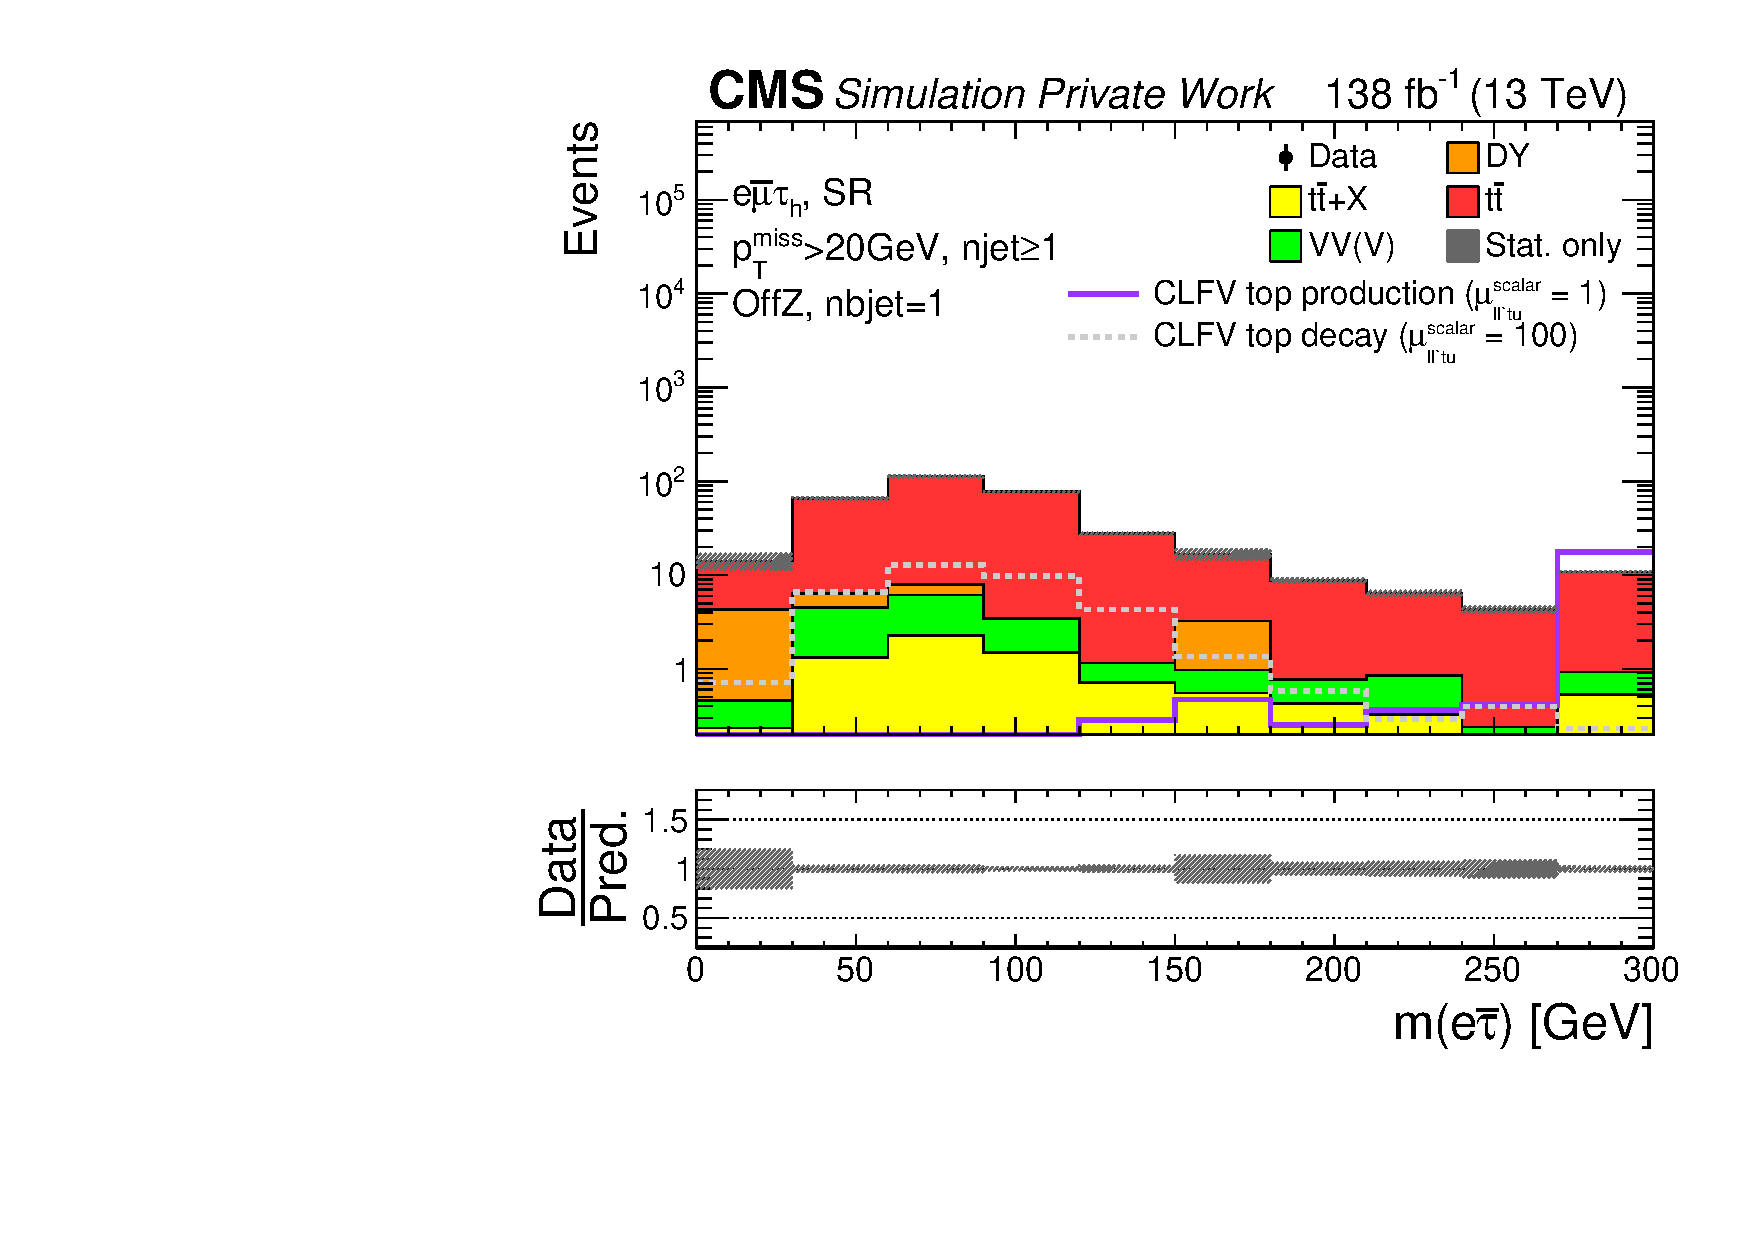
\includegraphics[width=0.33\textwidth]{figures/Part4/Evt/LFVetaM}&
 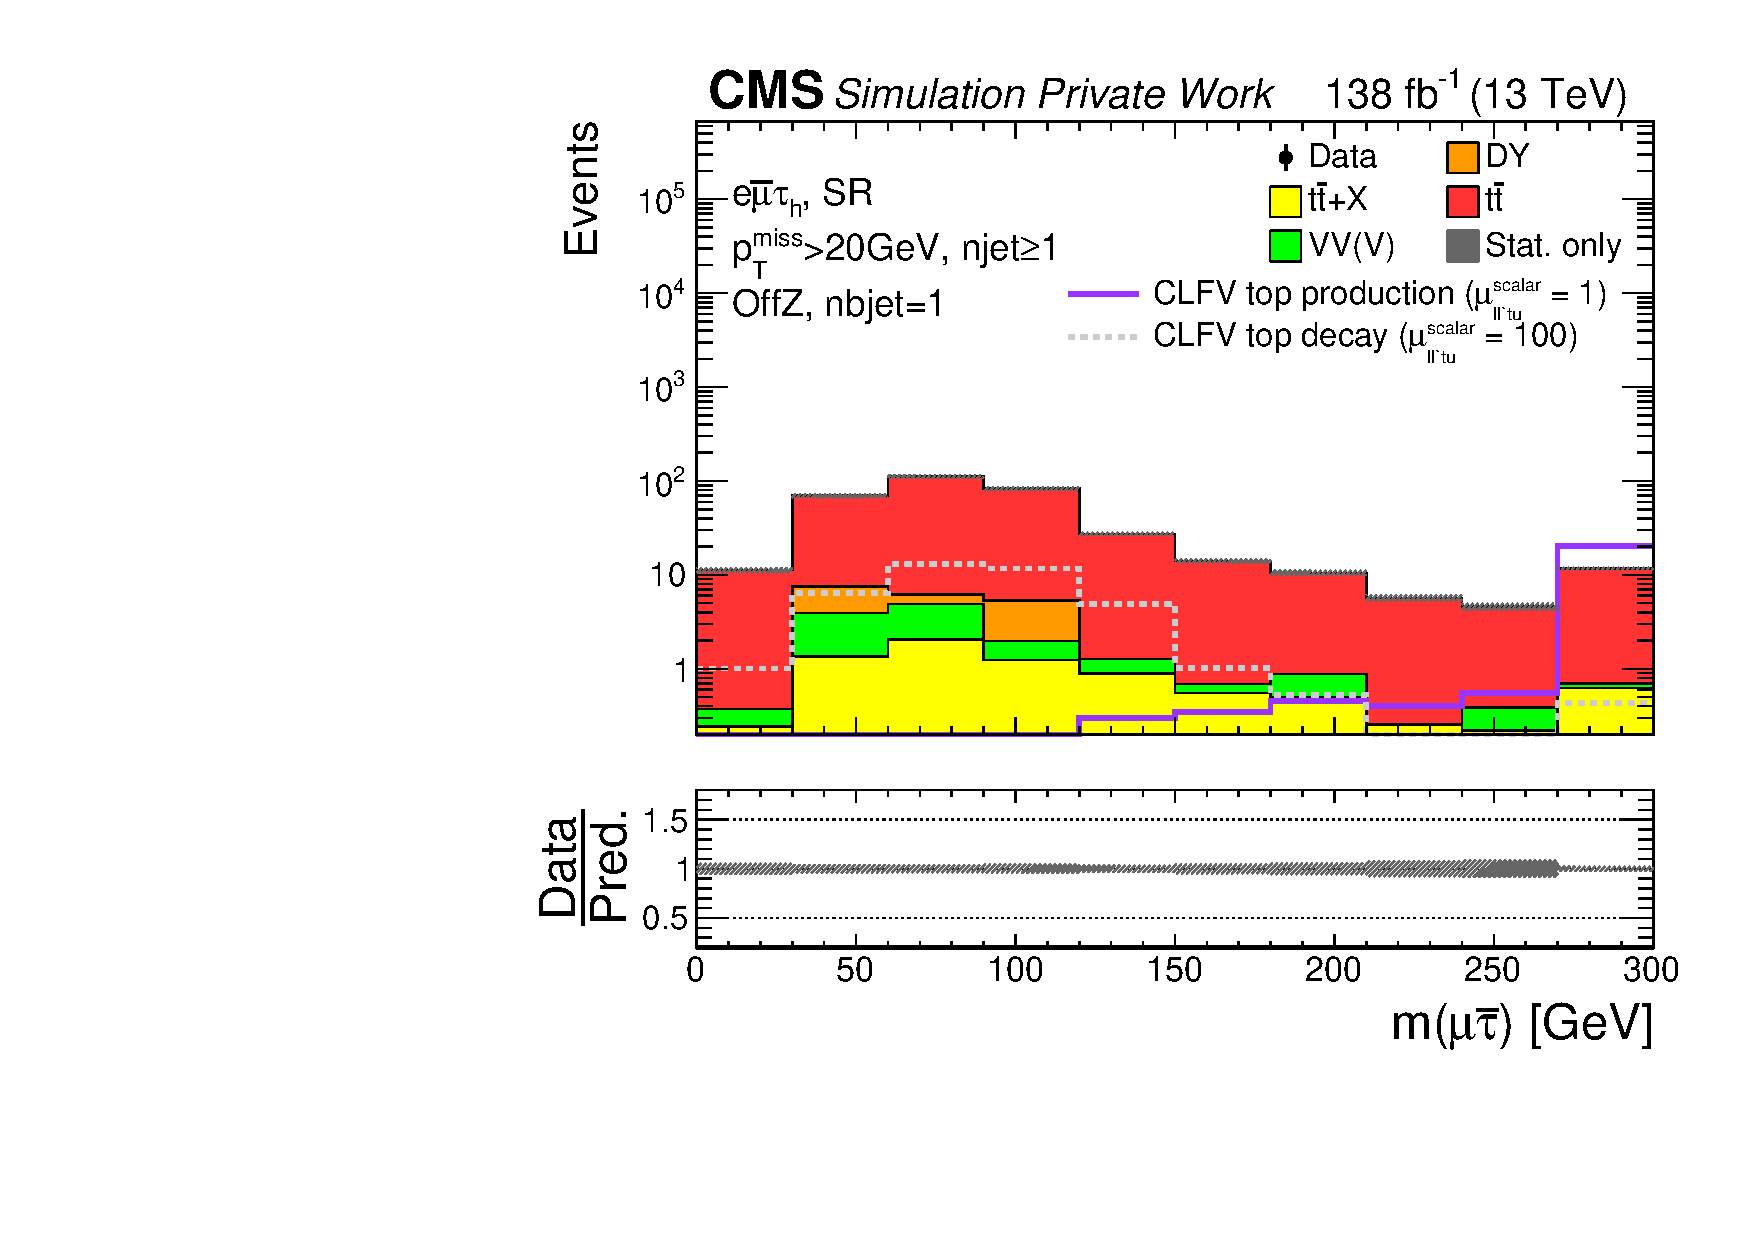
\includegraphics[width=0.33\textwidth]{figures/Part4/Evt/LFVmutaM}\\
 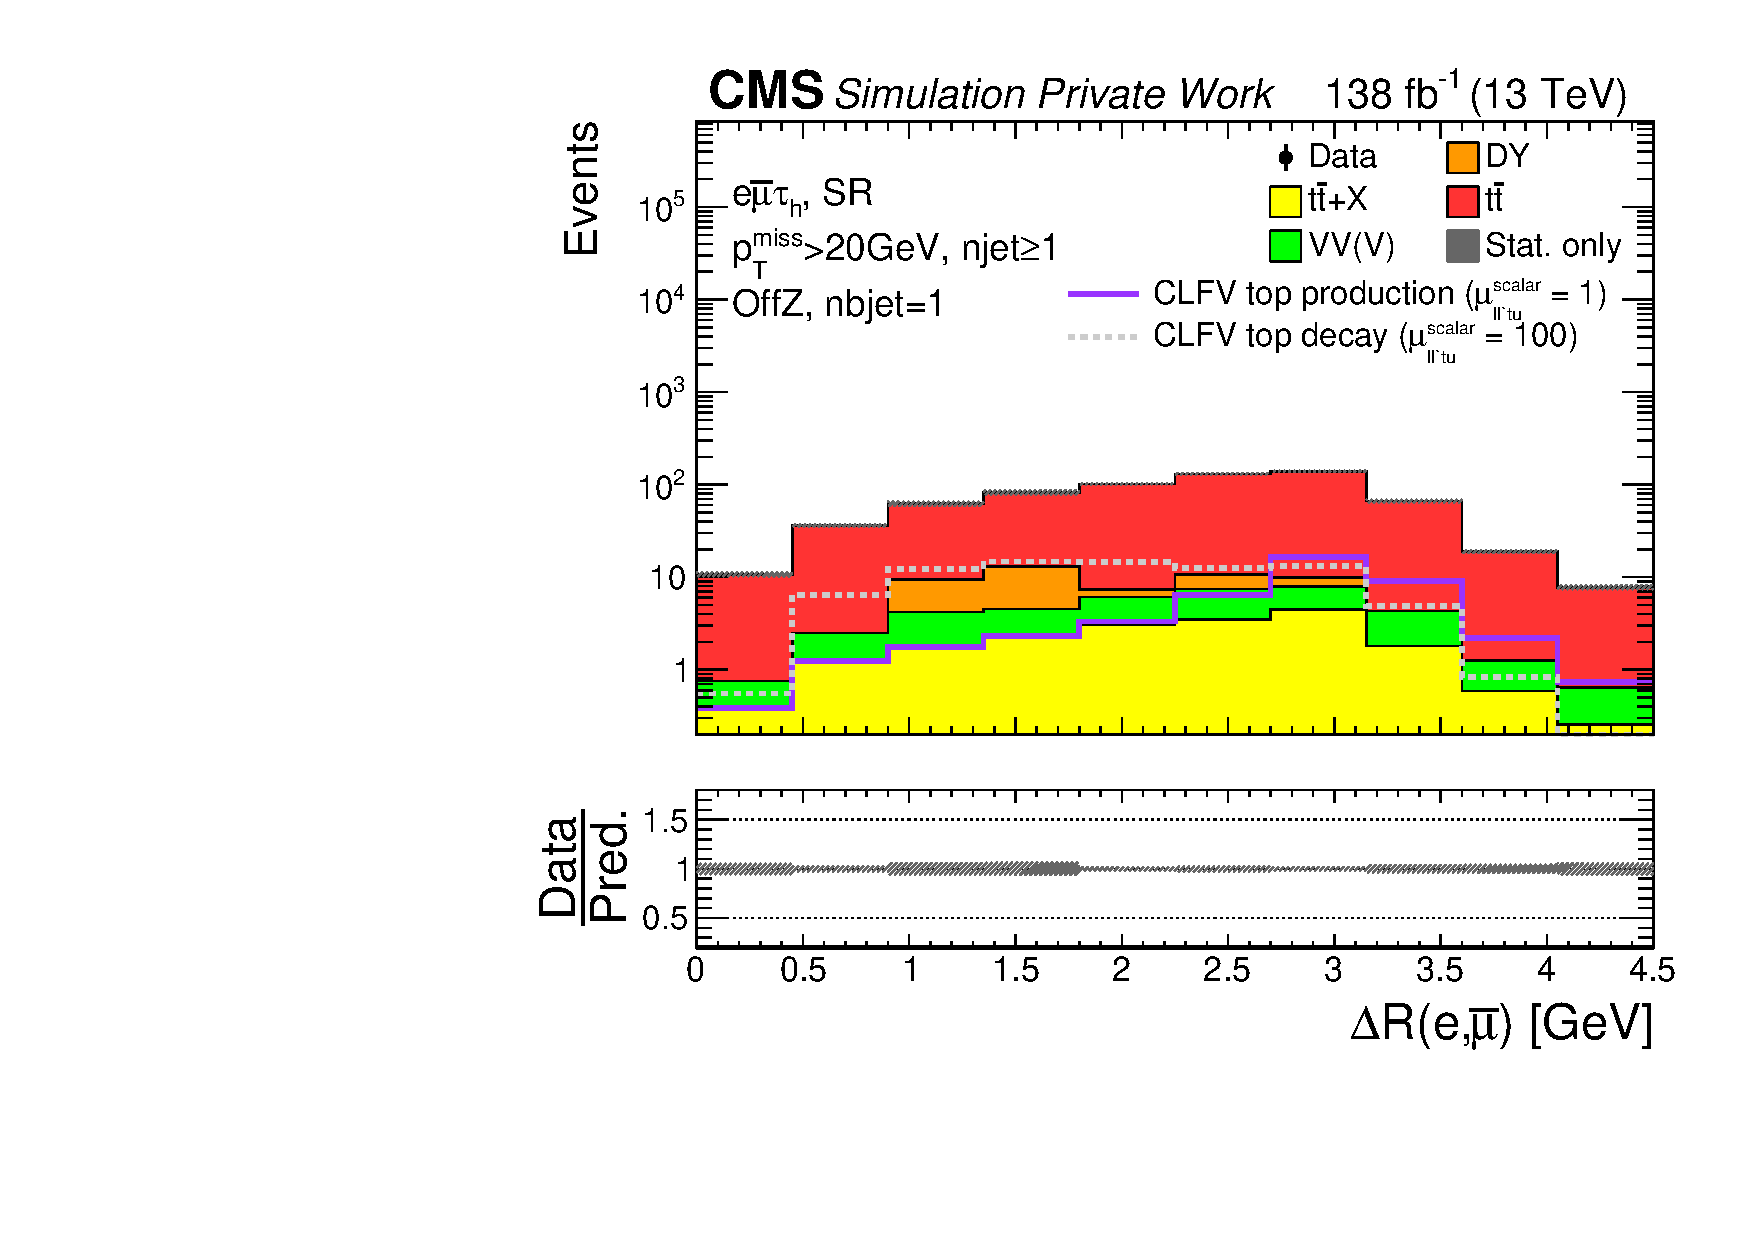
\includegraphics[width=0.33\textwidth]{figures/Part4/Evt/LFVemuDr}&
 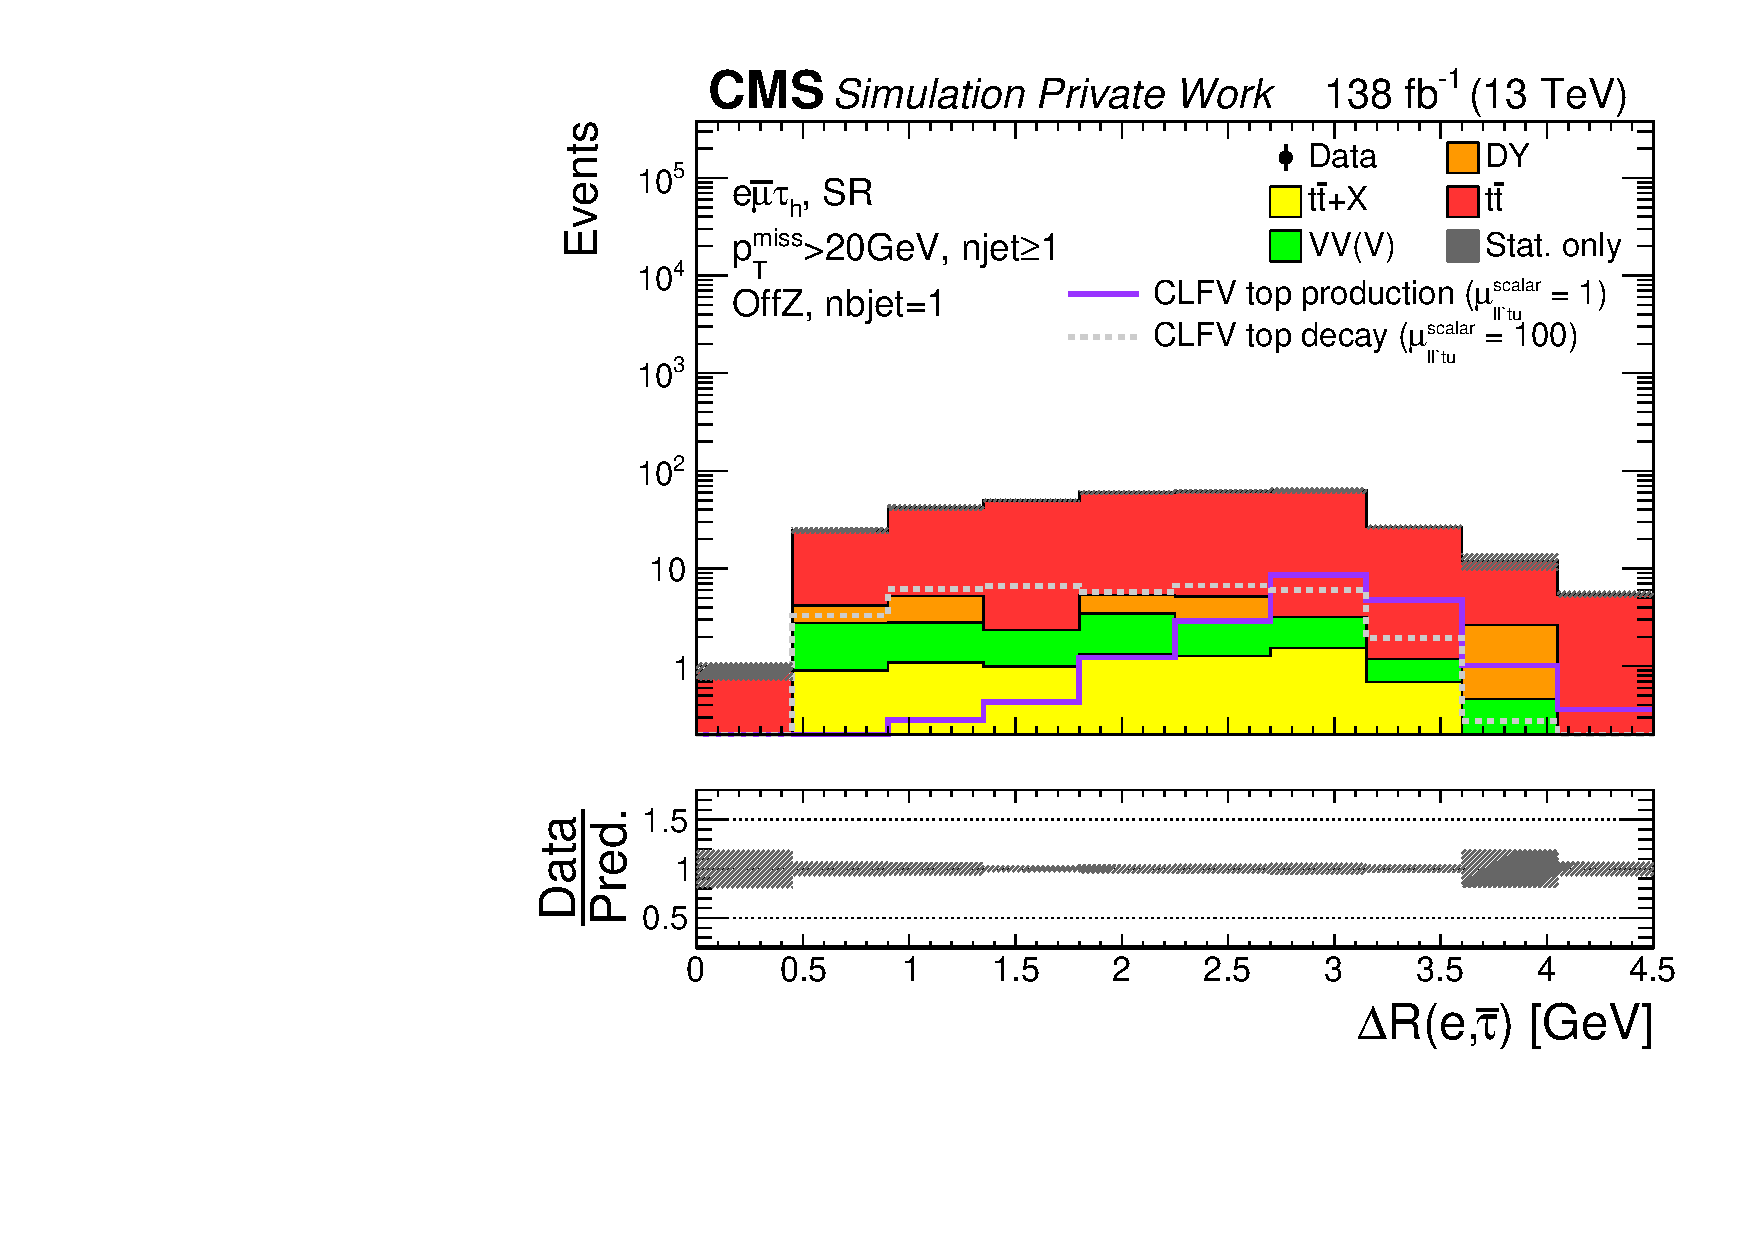
\includegraphics[width=0.33\textwidth]{figures/Part4/Evt/LFVetaDr}&
 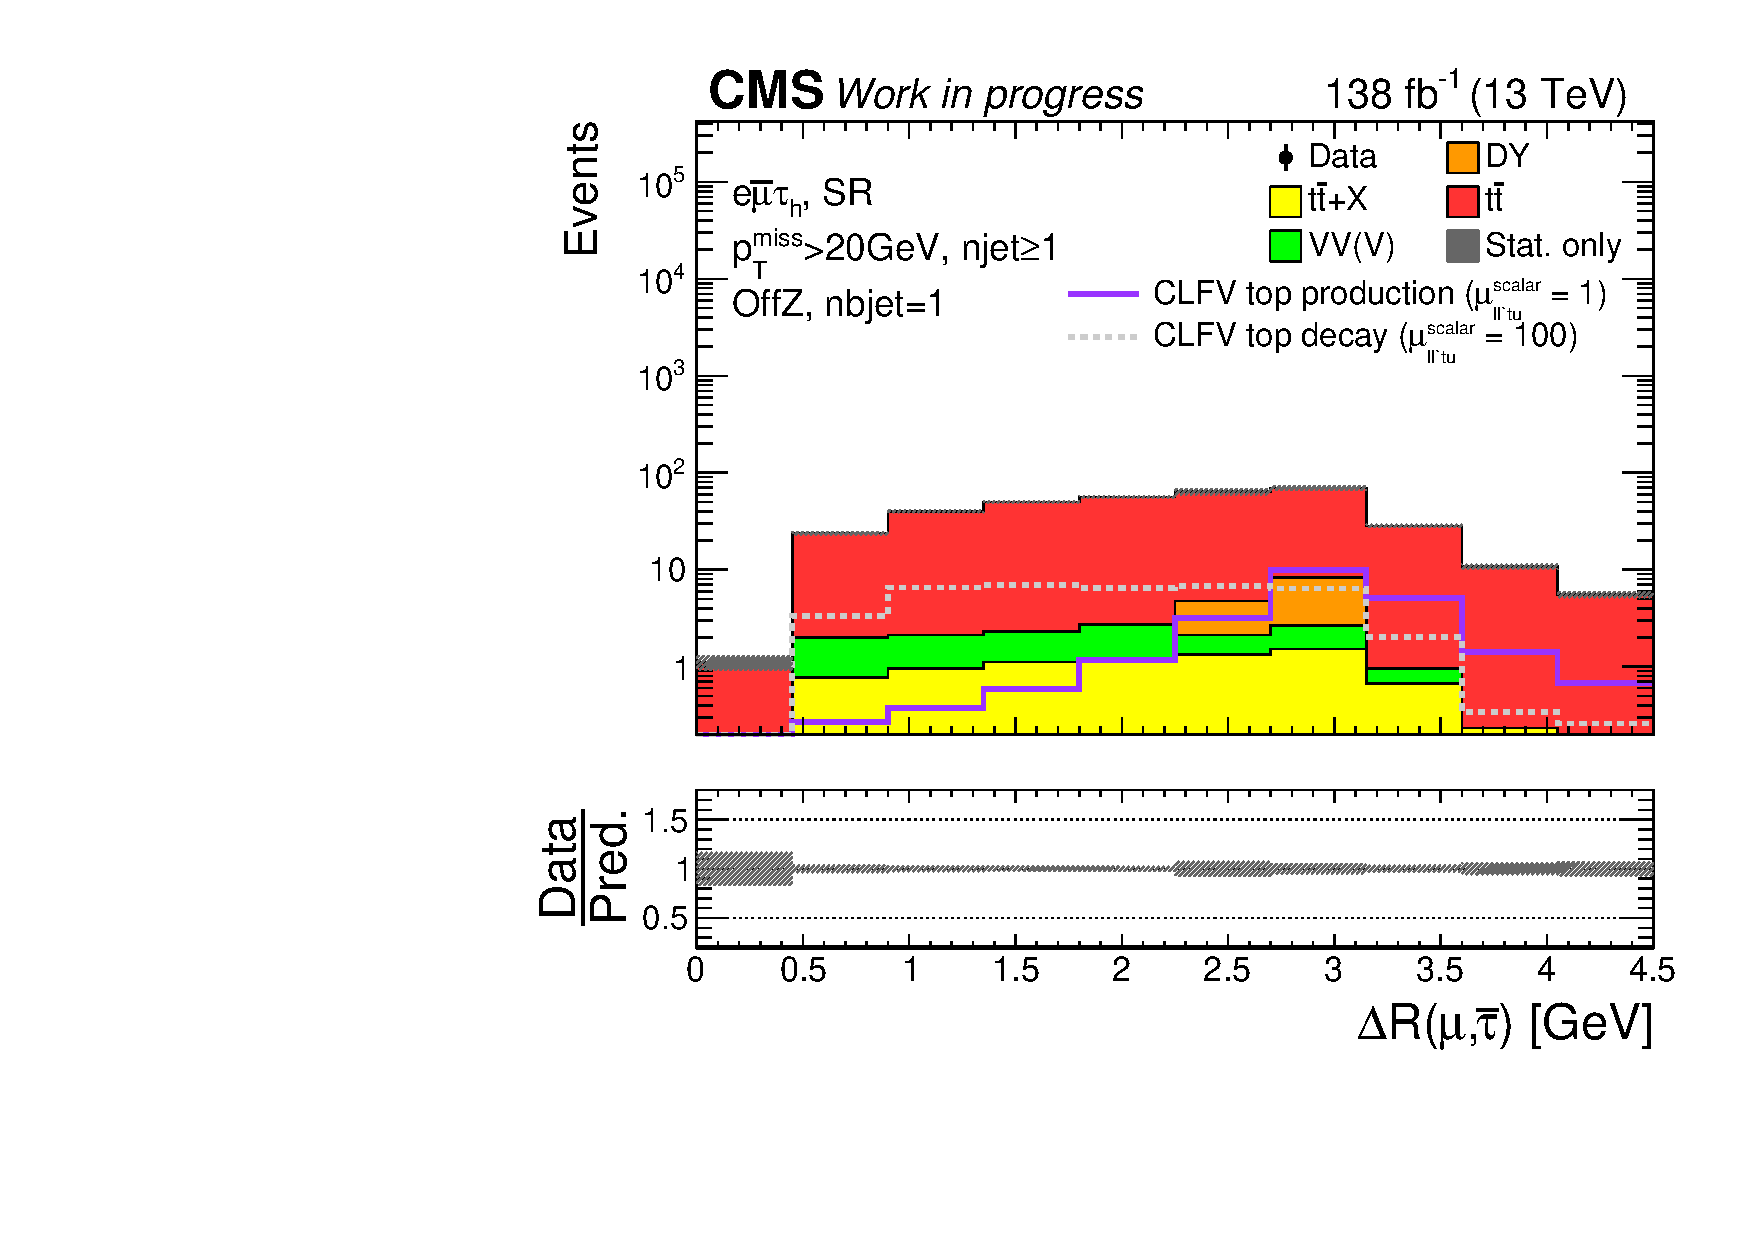
\includegraphics[width=0.33\textwidth]{figures/Part4/Evt/LFVmutaDr}\\
 \end{tabular}
 \caption{XX}
 \label{fig:LFVmass}
 \end{center}
 \end{figure}
%%%%%%%%%%%%%%%%%%%%%%%%%%%%%%%%%%%%%%%%%%%%%%%%%%
%%%%%%%%%%%%%%%%%%%%%%%%%%%%%%%%%%%%%%%%%%%%%%%%%%

\section{Drell-Yan Control Region}
\label{sec:DY_CR}

 \begin{figure}[tbh!]
 \begin{center}
 \begin{tabular}{cc}
 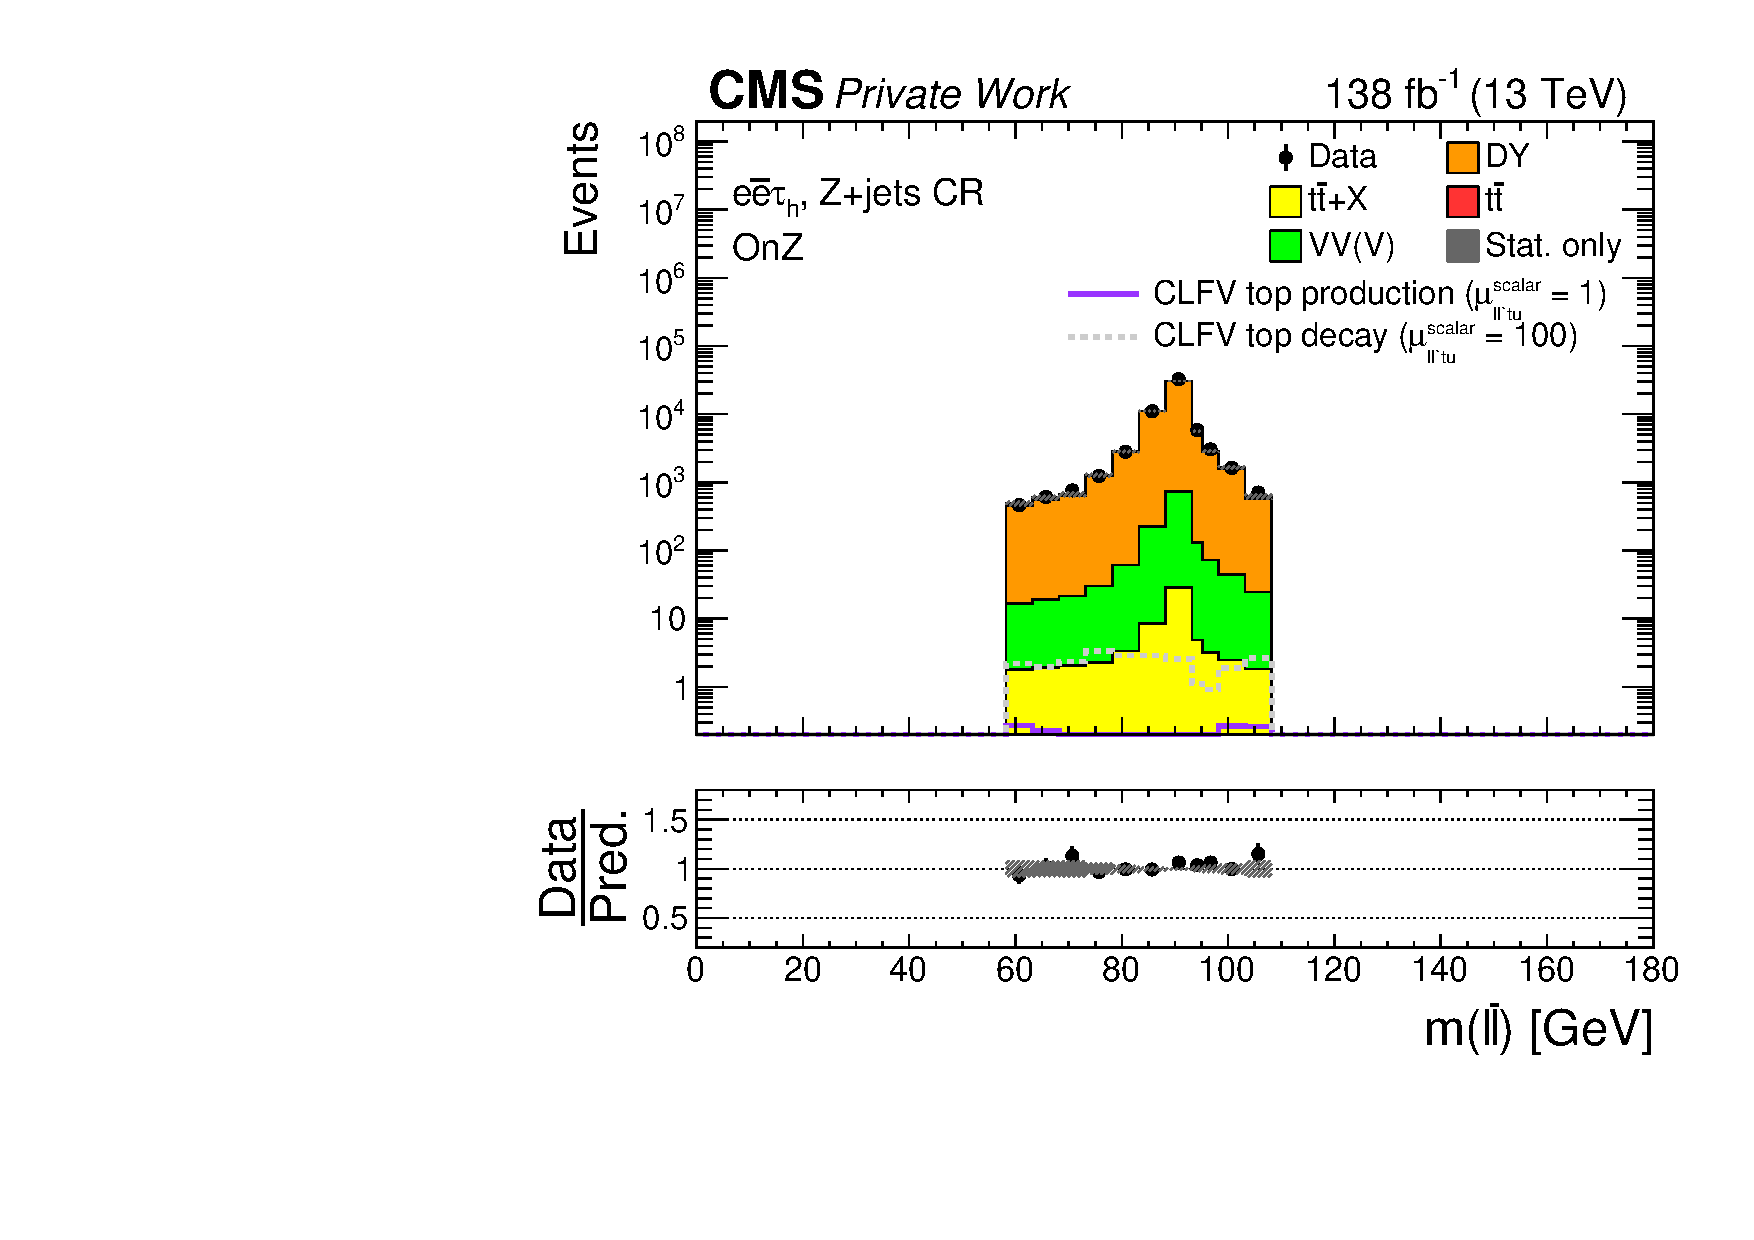
\includegraphics[width=0.48\textwidth]{figures/Part4/Evt/llM_OnZ_ee}&
 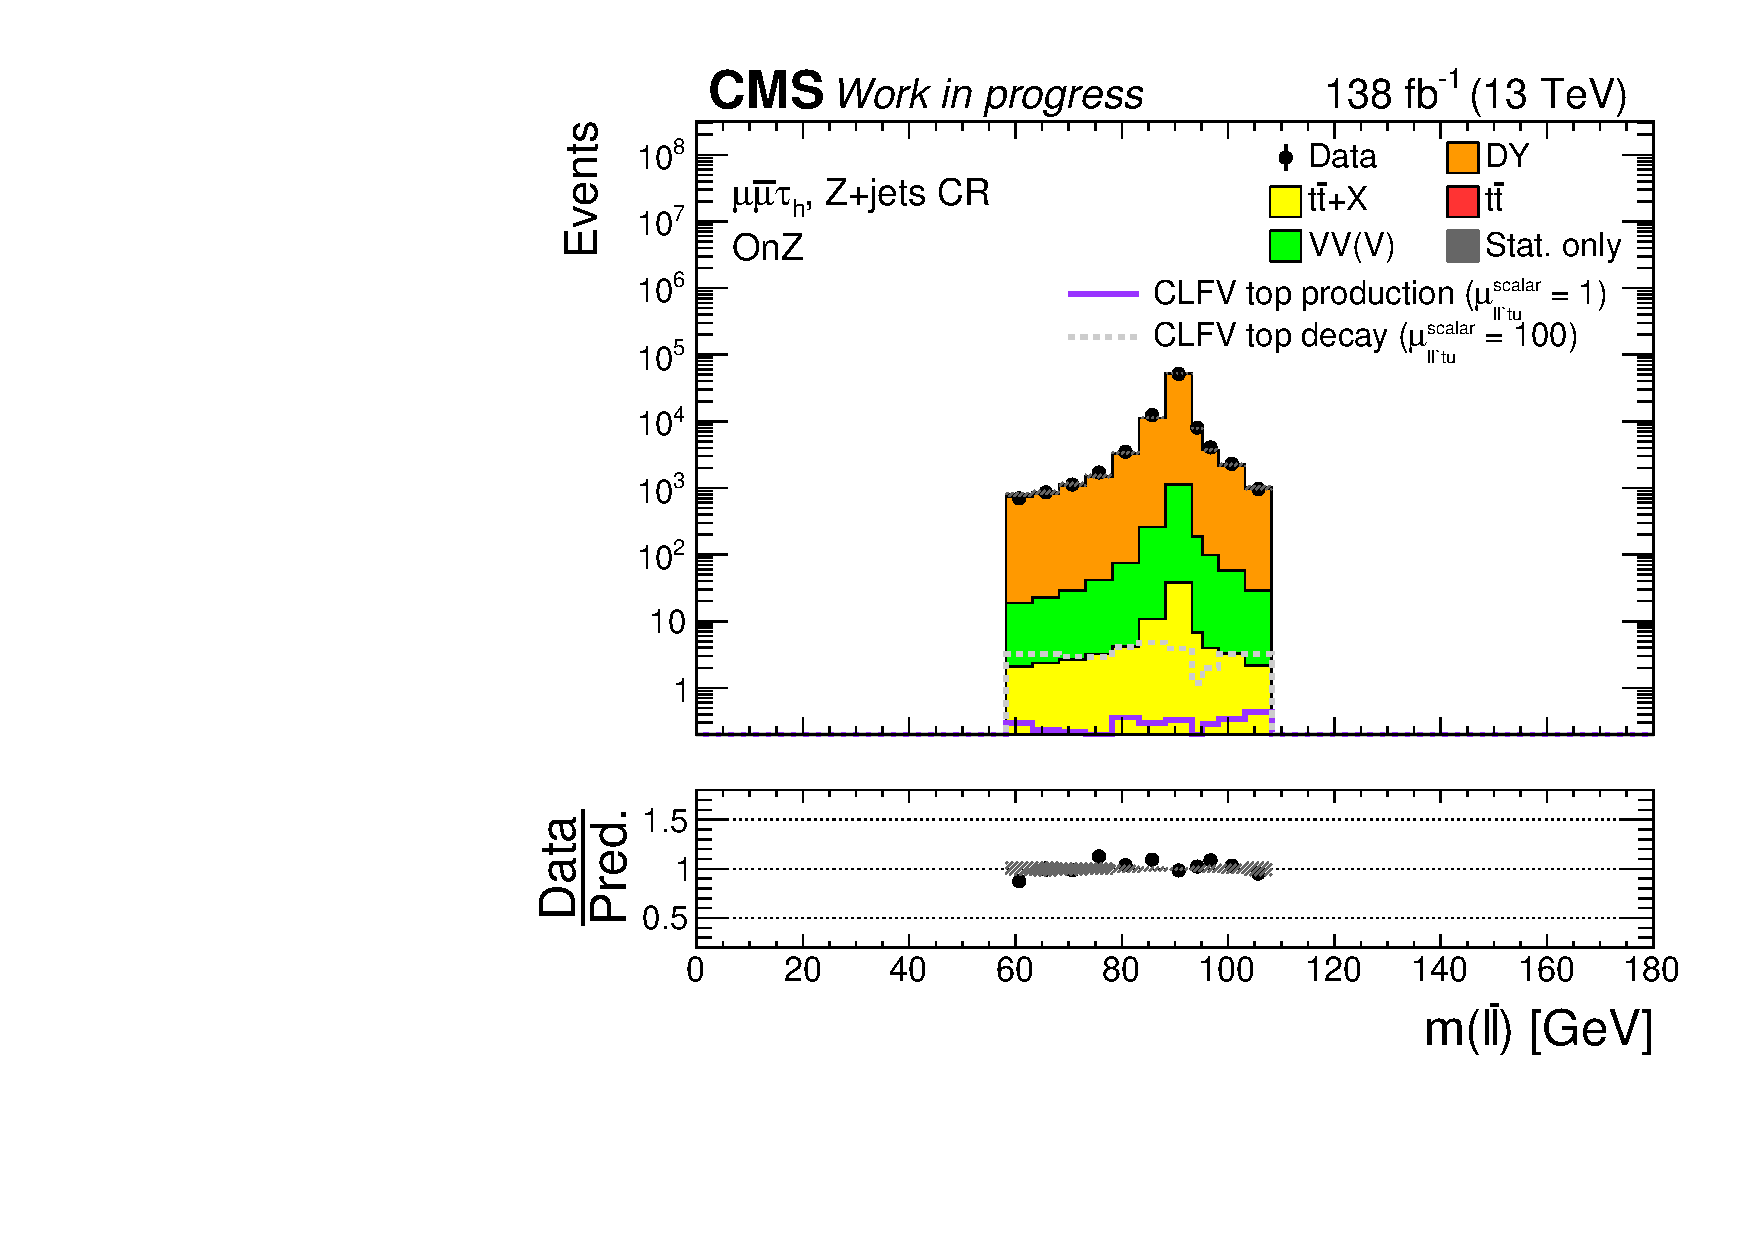
\includegraphics[width=0.48\textwidth]{figures/Part4/Evt/llM_OnZ_mumu}\\
  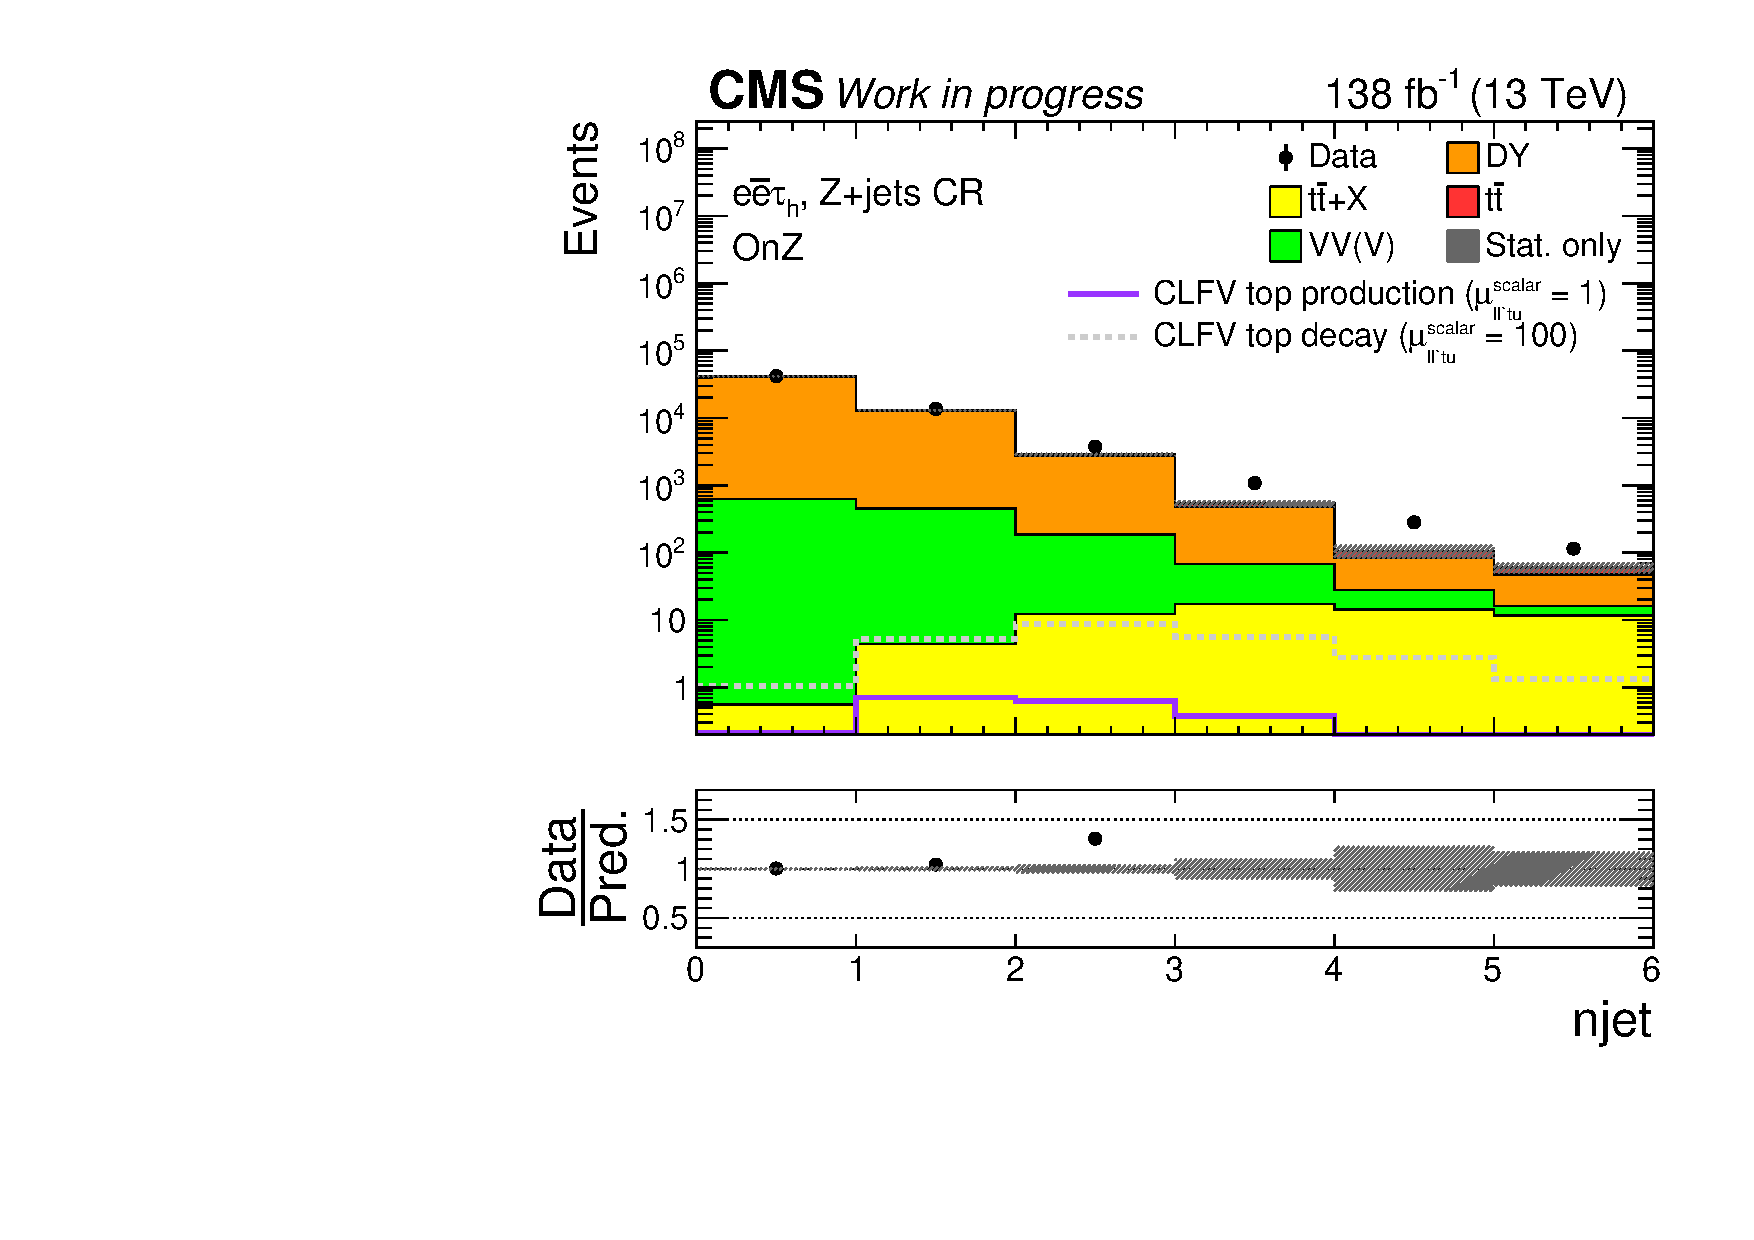
\includegraphics[width=0.48\textwidth]{figures/Part4/Evt/njet_OnZ_ee}&
 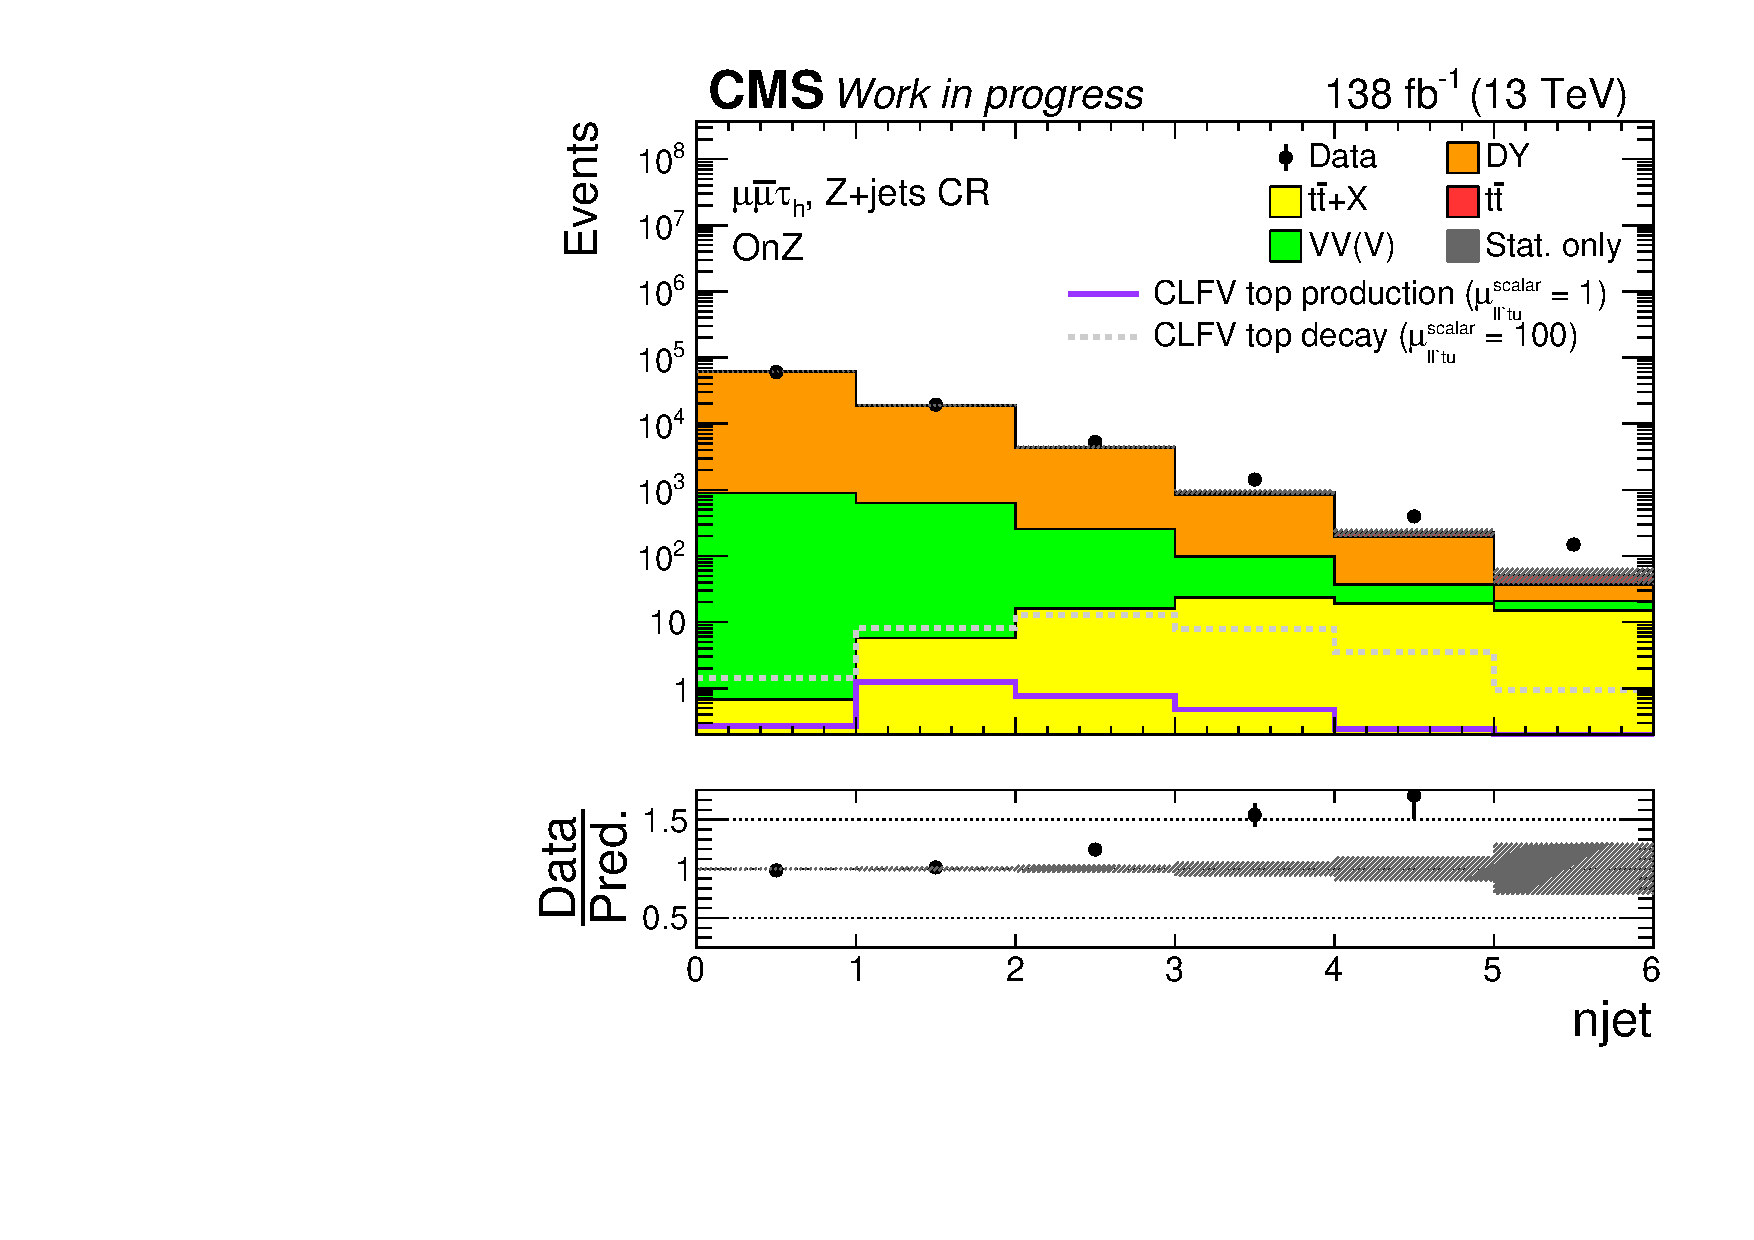
\includegraphics[width=0.48\textwidth]{figures/Part4/Evt/njet_OnZ_mumu}\\
 \end{tabular}
 \caption{XX}
 \label{fig:DY_CR}
 \end{center}
 \end{figure}